\documentclass{beamer}

\usepackage[utf8]{inputenc}
\usepackage{ngerman}

\usetheme{Warsaw}
%\usecolortheme[named=orange]{structure}
%\useinnertheme{rectangles}

\setbeamercovered{transparent}

\beamertemplatenavigationsymbolsempty

\title{Korallenriff}
\date{\today}
\institute{Friedrich Engels Gymnasium - Biologie}
\titlegraphic{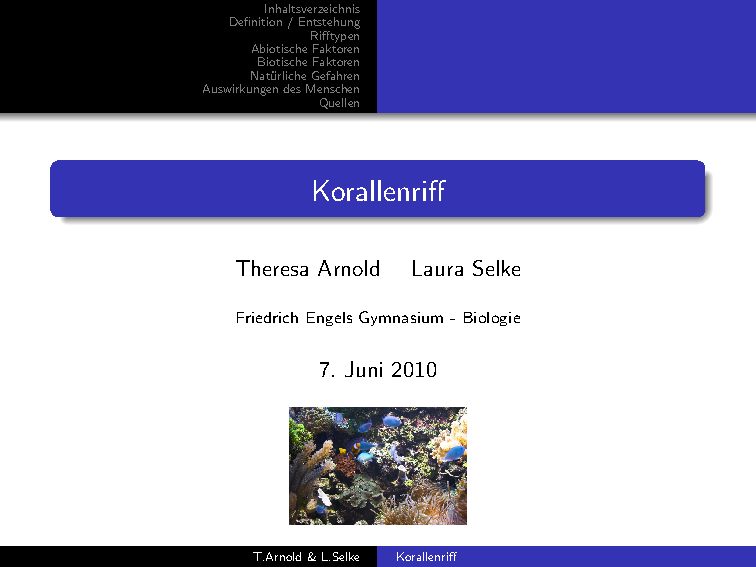
\includegraphics[width=3cm]{korallenriff.jpg}}
\author[T.Arnold \& L.Selke]{Theresa Arnold \and Laura Selke}


%\AtBeginSection{
    %\begin{frame}{}
        %\begin{block}{}
            %\titleref
        %\end{block}
    %\end{frame}
%}
\setbeamertemplate{sections/subsections in toc}[rounded] 
\setbeamercolor{section number projected}{fg=blue!10!white,bg=black}
\setbeamercolor{section in toc}{fg=blue!40!black}
\setbeamercolor{subsection in toc}{fg=black}

\begin{document}

%\setbeamertemplate{background canvas}[vertical shading][top=blue!30, bottom=red!30]



\begin{frame}
    \titlepage
\end{frame}

\section*{Inhaltsverzeichnis}
\begin{frame}{Inhaltsverzeichnis}
    \tableofcontents[pausesections]
\end{frame}

\section{Definition / Entstehung}
\frame{\begin{block}{}\begin{center}\Huge{\textbf{Definition / Entstehung}}\end{center}\end{block}}

\frame{\begin{center}
        \includegraphics[width=9cm]{Bilder/korallenriff_1}\\
        \begin{block}{}
            \center{Korallenriff}
        \end{block}
\end{center}}

\frame{\begin{center}
        \includegraphics[width=7.5cm]{Bilder/Steinkorallen_2}\\
        \begin{block}{}
            \center{Steinkorallen}
        \end{block}
\end{center}}

\frame{\begin{center}
        \includegraphics[width=7.5cm]{Bilder/koralle.jpg}\\
        \begin{block}{}
            \center{Koralle}
        \end{block}
\end{center}}

\frame{\begin{center}
        \includegraphics[width=9cm]{Bilder/Korallenpolyp_3}\\
        \begin{block}{}
            \center{Korallenpolyp}
        \end{block}
\end{center}}

\frame{
    \begin{columns}
        \column{.5\textwidth}
        \center{\includegraphics[width=5cm]{Bilder/Great_Barrier_Reef_4.png}}
        \column{.5\textwidth}
        \center{\includegraphics[width=5cm]{Bilder/great_barrier_reed_4.jpg}}
    \end{columns}
    \begin{block}{}
        \center{Great Barrier Reef}
    \end{block}
}

\section{Rifftypen}
\frame{\begin{block}{}\begin{center}\Huge{\textbf{Rifftypen}}\end{center}\end{block}}

    \subsection{Tropisches Korallenriff}
\frame{
    \begin{center}
        \includegraphics[width=4.5cm]{Bilder/Zoxanthelle_5.jpg}
    \end{center}
    \begin{block}{}
        \center{Zooxanthelle}
    \end{block}
}

    \subsection{Tiefwasserriff}
\frame{
    \begin{center}
        \includegraphics[width=7cm]{Bilder/azooxanthelle_6.jpg}
    \end{center}
    \begin{block}{}
        \center{Azooxanthelle}
    \end{block}
}

\section{Abiotische Faktoren}
\frame{\begin{block}{}\begin{center}\Huge{\textbf{Abiotische Faktoren}}\end{center}\end{block}}

\frame{
    \begin{center}
        \includegraphics[width=7cm]{Bilder/Licht.jpg}
    \end{center}
    \begin{block}{}
        \center{Licht}
    \end{block}
}

\frame{
    \begin{center}
        \includegraphics[width=1cm]{Bilder/Temperatur.png}
    \end{center}
    \begin{block}{}
        \center{Temperatur}
    \end{block}
}

\frame{
    \begin{center}
        \includegraphics[width=7cm]{Bilder/Salzgehalt.png}
    \end{center}
    \begin{block}{}
        \center{Salzgehalt}
    \end{block}
}

\frame{
    \begin{columns}
        \column{.5\textwidth}
        \center{\includegraphics[width=5cm]{Bilder/robuste_Koralle.jpg}}
        \begin{block}{}
            \center{robuste Koralle}
        \end{block}
        \column{.5\textwidth}
        \center{\includegraphics[width=5cm]{Bilder/filigrane_Koralle.jpg}}
        \begin{block}{}
            \center{filigrane Koralle}
        \end{block}
    \end{columns}
}

\section{Biotische Faktoren}
\frame{\begin{block}{}\begin{center}\Huge{\textbf{Biotische Faktoren}}\end{center}\end{block}}

\frame{
    \begin{center}
        \includegraphics[width=7cm]{Bilder/Zooplankton_7.jpg}
    \end{center}
    \begin{block}{}
        \center{Zooplankton}
    \end{block}
}

\begin{frame}[plain]
    \begin{figure}
        \includegraphics<1>[width=11.5cm]{Bilder/Symbiose.png}
        \includegraphics<2>[width=11.5cm]{Bilder/Symbiose01.png}
        \includegraphics<3>[width=11.5cm]{Bilder/Symbiose02.png}
        \includegraphics<4>[width=11.5cm]{Bilder/Symbiose03.png}
        \includegraphics<5>[width=11.5cm]{Bilder/Symbiose04.png}
        \includegraphics<6>[width=11.5cm]{Bilder/Symbiose05.png}
        \includegraphics<7>[width=11.5cm]{Bilder/Symbiose06.png}
        \includegraphics<8>[width=11.5cm]{Bilder/Symbiose07.png}
        \includegraphics<9>[width=11.5cm]{Bilder/Symbiose08.png}
        \includegraphics<10>[width=11.5cm]{Bilder/Symbiose09.png}
        \includegraphics<11>[width=11.5cm]{Bilder/Symbiose10.png}
        \includegraphics<12>[width=11.5cm]{Bilder/Symbiose11.png}
    \end{figure}
\end{frame}


\frame{
    \begin{columns}
        \column{.5\textwidth}
        \center{\includegraphics[width=5cm]{Bilder/Anemone_8.jpg}}
        \begin{block}{}
            \center{Anemone}
        \end{block}
        \column{.5\textwidth}
        \center{\includegraphics[width=5cm]{Bilder/Anemonenfisch_9.jpg}}
        \begin{block}{}
            \center{Anemonenfisch}
        \end{block}
    \end{columns}
}

\frame{
    \begin{center}
        \includegraphics[width=8cm]{Bilder/Nahrungspyramide.jpg}
    \end{center}
    \begin{block}{}
        \center{Nahrungspyramide}
    \end{block}
}


\frame{
    \begin{columns}
        \column{.5\textwidth}
        \center{\includegraphics[width=5cm]{Bilder/Phytoplankton_11.jpg}}
        \begin{block}{}
            \center{Phytoplankton}
        \end{block}
        \column{.5\textwidth}
        \center{\includegraphics[width=5cm]{Bilder/Seegras_11.jpg}}
        \begin{block}{}
            \center{Seegras}
        \end{block}
    \end{columns}
}

\frame{
    \begin{center}
        \includegraphics[width=7cm]{Bilder/Papageienfisch_10.jpg}
    \end{center}
    \begin{block}{}
        \center{Papageienfisch}
    \end{block}
}

\begin{frame}
    \begin{columns}
        \column{0.18\textwidth}
        \center{\includegraphics[width=2.8cm]{Bilder/Phytoplankton_11.jpg}}
        \column{0.02\textwidth}
        \column{0.18\textwidth}
        \column{0.02\textwidth}
        \column{0.18\textwidth}
    \end{columns}
    \begin{block}{}
        \center{Nahrungskette}
    \end{block}
\end{frame}

\begin{frame}
    \begin{columns}
        \column{0.18\textwidth}
        \center{\includegraphics[width=2.8cm]{Bilder/Phytoplankton_11.jpg}}
        \column{0.02\textwidth}
        \center{\includegraphics[width=0.8cm]{Bilder/pfeil.png}}
        \column{0.18\textwidth}
        \center{\includegraphics[width=2.8cm]{Bilder/koralle.jpg}}
        \column{0.02\textwidth}
        \column{0.18\textwidth}
    \end{columns}
    \begin{block}{}
        \center{Nahrungskette}
    \end{block}
\end{frame}

\begin{frame}
    \begin{columns}
        \column{0.18\textwidth}
        \center{\includegraphics[width=2.8cm]{Bilder/Phytoplankton_11.jpg}}
        \column{0.02\textwidth}
        \center{\includegraphics[width=0.8cm]{Bilder/pfeil.png}}
        \column{0.18\textwidth}
        \center{\includegraphics[width=2.8cm]{Bilder/koralle.jpg}}
        \column{0.02\textwidth}
        \center{\includegraphics[width=0.8cm]{Bilder/pfeil.png}}
        \column{0.18\textwidth}
        \center{\includegraphics[width=2.8cm]{Bilder/Papageienfisch_10.jpg}}
    \end{columns}
    \begin{block}{}
        \center{Nahrungskette}
    \end{block}
\end{frame}


\section{Natürliche Gefahren}
\frame{\begin{block}{}\begin{center}\Huge{\textbf{Natürliche Gefahren}}\end{center}\end{block}}

    \subsection{Fische als Räuber}
\frame{
    \begin{center}
        \includegraphics[width=7cm]{Bilder/Papageienfisch_12.jpg}
    \end{center}
    \begin{block}{}
        \center{Papageienfisch}
    \end{block}
}
    %Papageienfisch 12
\frame{
    \begin{center}
        \includegraphics[width=7cm]{Bilder/Dornenkrone_13.jpg}
    \end{center}
    \begin{block}{}
        \center{Dornenkrone}
    \end{block}
}
    %Dornenkrone

    \subsection{Korallenbleiche}
\frame{
    \begin{center}
        \includegraphics[width=5.5cm]{Bilder/Korallenbleiche_14.jpg}
    \end{center}
    \begin{block}{}
        \center{Korallenbleiche}
    \end{block}
}
    % Korallenbleiche ohne strich
\frame{
    \begin{center}
        \includegraphics[width=7cm]{Bilder/Korallenbleiche-_14.jpg}
    \end{center}
    \begin{block}{}
        \center{Korallenbleiche}
    \end{block}
}
    % Korallenbleiche mit strich

\section{Auswirkungen des Menschen}
\frame{\begin{block}{}\begin{center}\Huge{\textbf{Auswirkungen des Menschen}}\end{center}\end{block}}

    \subsection{Künstliche Korallenriffe}
\frame{
    \begin{center}
        \includegraphics[width=7cm]{Bilder/kunstliche_Korallenriffe_15.jpg}
    \end{center}
    \begin{block}{}
        \center{Künstliche Korallenriffe}
    \end{block}
}
    % kunstliche Korallenriffe
\frame{
    \begin{center}
        \includegraphics[width=7cm]{Bilder/Osborne_Riff_16.jpg}
    \end{center}
    \begin{block}{}
        \center{Osborne Riff}
    \end{block}
}
    % Osborne riff
    \subsection{Verschmutzung}
\frame{
    \begin{center}
        \includegraphics[width=7cm]{Bilder/verschmutztes_Korallenriff_17.jpg}
    \end{center}
    \begin{block}{}
        \center{Verschmutztes Korallenriff}
    \end{block}
}
    % verschmutztes Korallenriff
\frame{
    \begin{center}
        \includegraphics[width=7cm]{Bilder/Tourismus_18.jpg}
    \end{center}
    \begin{block}{}
        \center{Tourismus}
    \end{block}
}
    % Tourismus
\frame{
    \begin{center}
        \includegraphics[width=7cm]{Bilder/Oelteppich_18.jpg}
    \end{center}
    \begin{block}{}
        \center{Ölteppich}
    \end{block}
}
    % Oelteppich
\section*{Quellen}
\frame{\begin{block}{}\begin{center}\Huge{\textbf{Quellen}}\end{center}\end{block}}

\frame{
    \begin{block}{Internet}
    \begin{tiny}

http://www.planet-wissen.de/natur\_technik/meer/korallenriffe/symbiosen\_am\_riff.jsp\\
http://www.planet-wissen.de/natur\_technik/meer/korallenriffe/index.jsp\\
http://www.jadestern.de/index.php?id=174\\
http://www.guidobauersachs.de/referate/nako.htm\\
http://de.wikipedia.org/wiki/Korallenriff\#Atolle\\
http://www.starfish.ch/Korallenriff/Meer.html\\
http://www.referate10.com/referate/Biologie/22/Referat-Das-Okosystem-Korallenriff-reon.php\\
http://www.mpi-bremen.de/Oekosystem\_Korallenriff.html\\
http://www.bg-bab.ac.at/jordan/german/korallen.htm\\
http://mypics.at/bilder/schoenbrunn/aquarien/korallenriff-4033.jpg.html\\
http://www.spiegel.de/wissenschaft/natur/0,1518,685398,00.html\\
http://www.suedseetraeumereien.de/Leben\_im\_Korallenriff\_2.html\\
http://archiv.korallenriff.de/\\
\end{tiny}
\end{block}
    \begin{block}{Bücher}
    \begin{tiny}
Karibik - Ein Unterwasserparadis\\
Wunderwelt des Meeres\\
Leben im Meer - Wie es ist, Wie es wurde, Wie es werden kann\\
\end{tiny}
\end{block}
\pause
}

\end{document}
